\documentclass{article}

\usepackage[ngerman]{babel} 

\usepackage[T1]{fontenc}
\usepackage{lmodern}
\usepackage[utf8]{inputenc}
\usepackage{graphicx}
\usepackage{amsmath}
\usepackage{amssymb}
\usepackage{amsthm} 
\usepackage{wasysym}
\usepackage[justification=centering]{caption}
\usepackage[parfill]{parskip}
\usepackage[left=3cm,right=3cm,top=2cm,bottom=2cm,includeheadfoot]{geometry}
\usepackage{subfig}
\usepackage{units}
\usepackage{subscript}
\usepackage[ruled,german]{algorithm2e}
\usepackage{textcomp}
\usepackage{tikz}
\usepackage{listings}
\usepackage{url}

\lstset{
  language=C,
  tabsize=4,
  captionpos=b,
  numbers=left,
  commentstyle=\color{green},
  backgroundcolor=\color{white},
  numberstyle=\color{gray},
  keywordstyle=\color{blue} \textbf,%otherkeywords={xdata},
  keywords=[2]{xdata},
  keywordstyle=[2]\color{red}\textbf,
  identifierstyle=\color{black},
  stringstyle=\color{red}\ttfamily,
  basicstyle = \ttfamily \color{black} \footnotesize,
  showstringspaces=false ,
  moredelim=[is][\color{yellow}]{|}{|},
}

\usetikzlibrary{shapes}

\newtheorem{satz}{Satz} 

\newcommand{\BigO}[1]{\ensuremath{\operatorname{O}\left(#1\right)}}
\newcommand{\subs}[2]{#1\textsubscript{#2}}

\usepackage[sortcites=true, style=alphabetic,natbib=true]{biblatex}

\bibliography{bibliography}

%Autornamen in Bibliography fett
\AtBeginBibliography{\renewcommand*{\mkbibnamelast }[1]{\textbf{#1}}}
\AtBeginBibliography{\renewcommand*{\mkbibnamefirst }[1]{\textbf{#1}}}

\title{Manganernte auf dem pazifischen Meeresgrund}
\date{\today}
\author{Jan-Christoph Klie \hspace{2cm} Stephan Alaniz Kupsch \\
\url{jck@mrklie.com} \hspace{2cm} \url{stephan.alaniz@gmail.com} \\
DHBW Mannheim }


\begin{document}
% Title page

\maketitle
\tableofcontents 
\newpage

% ############################################
\section{Problembeschreibung und -analyse}

\subsection{Problembeschreibung}

Aufgabe war es, Roboter zu simulieren, die allein auf sich gestellt auf dem
pazifischen Meeresboden Mangan sammeln und sich nach einer gewissen Zeit 
an einem gemeinsamen Punkt treffen.

Im weiteren wird ein kurzer Überblick über mögliche Lösungen gegeben, welche
warum implementiert wurde, und wie die Theorie dahinter aussieht. Schließlich
wird noch diskutiert, wie gut der gewählte Ansatz schließlich war und wie es
mit mehr Zeit (noch) besser gemacht werden kann.

\subsection{Annahmen über das Problem}

Es wurden Annahmen über die Eigenschaften des roblem  gemacht, wo es keine
Beschreibung/Limitierung gab. Diese sind im Folgenden:

\begin{itemize}
\item Roboter sind punktförmig
\item Roboter können in der Bewegung saugen
\item Es gibt keine Beschränkung, wie viele Roboter sich in einem Punkt befinden
\item Kommunikation ist instantan und ohne Berechnungszeit (Senden wie Empfangen)
\item Art der Kommunikation zwischen Robotern ist unbeschränkt (es kann alles übertragen werden)
\item Roboter haben unbeschränkt viel Speicher
\end{itemize}

\subsection{Disclaimer}

Die Einschränkungen, die mit dem Problem kommen, wurden nicht simuliert. Nur deren
Auswirkungen wurde berücksichtigt. 

% ############################################
\clearpage
\section{Vorgehensmodell und Entwicklung}

Die Entwicklung hat sich in zwei große Phasen geteilt. Beide hatten ihr eigenens Vorgehensmodell,
welche im Folgenden beschrieben werden:

\subsection{Ideenfindung}

Die erste Phase hat damit begonnen, mögliche Kanditaten für eine Lösung zu finden. Die Früchte dessen
sind in Kapitel \ref{sec:probrems} zu finden. Wichtig war, sich nicht auf einen Ansatz zu versteifen und
sofort zu implementieren, sonder Für und Wider abzuwägen. Im Laufe dessen sind immer neue Ideen gekommen,
viele sind verworfen worden. Schließlich hat man sich für einen Ansatz entschieden, der möglichst schnell
ein Ergebnis liefern sollte und eine Grundlage für alle späteren Entwicklungen bildet. Als sich dann
herauskristallisiert hat, welcher Ansatz am geeignetsten war, wurde schließlich Phase Zwei eingeläutet,
die Entwicklung an sich.

\subsection{Design-Ziele}

Bevor jedoch implementiert wurde, wurden einige Richtlinien und Ziele definiert, wie genau entwickelt werden
soll. Diese werden im folgenden beschrieben:

\begin{description}
\item[Keep it simple] \hfill \\ Die Lösung sollte so einfach wie möglich gehalten sein. So wenig Abstraktion wie möglich, so viel wie nötig. Nichts implementieren, was nicht benötigt wird (z.B. Interfaces für womöglich benötigte Komponenten)
\item[Rapid Prototyping] \hfill \\ Lieber schnell einen Prototypen schreiben und gucken, ob es überhaupt funktionieren kann. Im Laufe
dieser Arbeit sind so vier oder fünf lauffähige Lösungen entstanden, und nur die letzte wurde so bereinigt und optimiert. Ziel
war, Zeit zu sparen, was auch erreicht wurde.
\item[Getrennt marschieren - vereint schlagen] \hfill \\ Es wurde versucht, Komponenten möglichst unabhängig zu entwickeln. Da viele 
der verwendeten Algorithmen ohne weiteres Stand-Alone getestet und implementiert werden konnten, wurde erst ganz am Schluss
integriert. So konnte ohne Probleme Schnittstellen und Datenstruktueren vollkommen geändert werden, ohne Änderungen an anderer
Stelle nach sich zu ziehen.
\item[Not reinventing the square wheel] \hfill \\ Fast alles an Standardbibliotheken wurde bereits entwickelt, und zwar besser, als man es
selbst könnte. Daher wurde lieber und ohne Zögern auf externe Module gesetzt.
\item[Optimize last] \hfill \\ Da viel Code geschrieben wird, der am Ende nicht mehr benutzt wird, wurde erst in der letzten Iteration
auf Performance geachtet. 
\item[90 \% thinking, 10 \% coding] \hfill \\ Die Zeit, die mit Programmierung an sich verbraucht wurde, hat nur einen geringen Anteil an
der Gesamtzeit. Daher wurde viel mehr Wert auf gute Ideen zum Anfang hin gelegt.
\item[Wenn unklar, abstrahiere] \hfill \\ Viele Detailentscheidungen wurden erst spät getroffen oder laufend geändert. Diese wurden so
implementiert, dass sie leicht austauschbar sind. Beispiel dafür ist die Modellierung des Meeresbodens. Im letzten Schritt
wurden diese Abstraktionen dann entfernt.
\end{description}

\subsection{Nicht-Ziele}

Es wurde keinen Wert darauf gelegt, eine ästethisch schöne Benutzeroberfläche zu entwickeln. Ziel war nur, dass sie Benutzerfreundlich ist.

\subsection{Entscheidungen}

Einige wichtige Entscheidungen wurden schon in der Beschreibung der Implementierung aufgezählt. Im Folgenden werden nun
noch

\begin{description}
\item[Python] \hfill \\ Python als Programmiersprache hat viele Vorteile. Zum einen ist es extrem viel einfacher, Protoypen zu schreiben,
da man im Allgemeinen viel weniger Code für Funktionalität braucht wie für vergleichbare andere Sprachen. Außerdem kommt Python 
``batteries included'', d.h. es gibt sehr viele externe Pakete, die sich einfach installieren lassen. Schließlich kann Python
als Duct Tape für nativen Code eingesetzt werden, was sich im Laufe des Projektes als äußerst praktisch erwiesen hat.
\item[Matplotlib] \hfill \\ Matplotlib ist ein Paket, welches für das Plotten von Daten zuständig ist. Außerdem kann es diese auch animieren. Es ist kein vergleichbares Paket in anderen Programmiersprachen bekannt, was so vielseitig visualisieren kann, und somit ein weiterer Grund für Python als Grundlage 
\item[Numpy] \hfill \\ Numpy bietet schnelle, native Datenstrukturen für N-Dimensionale Arrays an. Es ist Grundlage für die gespeicherten Daten. Diese Arrays können von Python aus an C-und-C++-Code übergeben werden, wo dann performant Number Crunching betrieben werden kann. Außerdem ist es gut für Rechenoperationen auf Matrizen, vergleichbar da mit MATLAB.
\item[Ipython notebook] \hfill \\ Zum Prototyping wurde eine Webanwendung benutzt, Ipython notebook genannt. Dort kann im Browser Python geschrieben werden und Matplotlib-Graphiken angezeigt werden. Somit kann das Arbeitsergebnis einfach geteilt werden. Beispiel dafür ist eine statische Version aus den Anfängen des Projektes: \url{http://goo.gl/z6B1N8}
\item[Cython] \hfill \\ Cython ist ein Python-Modul, welches eine Schnittstelle zwischen Python und C/C++ bietet. So ist die Logik des Erntens in C++ geschrieben (Laufzeit ist so von 200s auf unter 10s gefallen), und wird nur von Python aufgerufen.
\item[Git+Github] \hfill \\ Unverzichtbar mittlerweile ist die Versionsverwaltung von Sourcecode, vor allem, wenn mit mehreren Entwicklern zusammengearbeitet wird. 
\end{description}

% ############################################
\clearpage
\section{Problembetrachtung}
\label{sec:probrems}

Das Problem kann unter vielen verschiedenen Blickwinkeln betrachtet 
werden. Je nachdem, in welcher Domäne der Informatik
es eingeordnet wird, gibt es unterschiedliche Lösungsansätze.

In diesem Abschnitt wird kurz beschrieben, welche Ansätze
erdacht wurden, welches deren Vor- und Nachteile sind, und
für welche schließlich ausgewählt wurden.

\subsection{Graphenproblem}

\subsubsection{Graphendefinition}

Aus der zugrunde liegenden Umgebung aus quadratischen Zellen 
(beschrieben in Kapitel 4 [ref?]) lässt sich ein Graph erstellen, 
bei dem jeder Knoten einer Zelle entspricht und über eine Kante zu 
jeder Nachbarzelle verbunden ist. Da sich ein Roboter in jede 
beliebige Richtung bewegen kann, handelt es sich dabei um einen 
bidirektionalen Graphen. Kanten zwischen zwei Knoten besitzen 
eine Gewichtung, je nachdem, ob ein Feld bereits besucht wurde oder 
nicht. Zu einem Knoten, der bereits besucht wurde, kann somit jede 
auf ihn gerichtete Kante die Gewichtung 0 besitzen. Ein noch nicht 
besuchter Knoten hat dahingegen Kanten mit einer Gewichtung von 1 
die auf ihn zeigen.

\subsubsection{Problembeschreibung}

Es wird angenommen, dass die Position von einem Roboter und die 
Position des Ziels bekannt sind. Eine relative Position ist hier 
vollkommen ausreichend. Nun soll der Pfad gefunden werden, der 
in einer vorgegebenen Anzahl an Schritten (gleichzusetzen mit der 
vorhandenen Missionszeit) zum Ziel führt und dabei so viele 
unbesuchten Knoten wie möglich durchquert. Der Einfachheit halber
wird für jeden Roboter sequentiell der beste Weg gesucht.

\subsubsection{Lösungsansätze}

\paragraph{Depth Limited Search}

Depth Limited Search (beschränkte Tiefensuche) ist ein Suchalgorithmus, 
bei dem Baum oder ein Graph erst in der Tiefe und anschließend in der 
Breite durchsucht wird. Zusätzlich besitzt der Algorithmus eine feste 
Tiefe. Das heißt, dass der Algorithmus alle Pfade durchsucht, die die 
maximale Tiefe nicht überschreitet. Von jedem Node kann so bei einem 
Schritt zu einem der vier Nachbarn gegangen werden. Der folgende Pseudocode
beschreibt, wie Depth Limited Search funktioniert.

\begin{lstlisting}[frame=single, language=C]  % Start your code-block

DLS(node, goal, depth) {
  if ( depth >= 0 ) {
    if ( node == goal )
      return node

    for each child in expand(node)
      DLS(child, goal, depth-1)
  }
}
\end{lstlisting}

Bezogen auf einen Roboter wird die aktuelle Position (\texttt{node}) , das Ziel
(\texttt{goal}) und die Missionszeit (\texttt{depth}) dem Algorithmus übergeben. Da Depth
Limited Search ursprünglich terminiert, sobald das Ziel gefunden wurde, muss der
Algorithmus dahingehend modifiziert werden, sodass er alle möglichen Pfade
durchsucht und sich den besten merkt.

\begin{lstlisting}[frame=single, language=C]
DLS(node, goal, depth, path_so_far) {
  if ( depth >= 0 ) {
    if ( node == goal )
      path_so_far.append(node)
      check_for_path_score(path_so_far)
      path_so_far.pop()

    for each child in expand(node)
      path_so_far.append(node)
      DLS(child, goal, depth-1, path_so_far)
      path_so_far.pop()
  }
}
\end{lstlisting}

Die modifizierte DLS durchsucht nun alle möglichen Pfade,
berechnet in \texttt{check\_for\_path\_score()}, wie viele unbesuchten Knoten durchlaufen
werden und speichert zugleich den besten Pfad, den er findet.

Der Hauptvorteil von Depth Limited Search ist, dass der Algorithmus definitiv den
best möglichen Pfad zum Ziel im gegebenen Szenario findet. Der entscheidene
Nachteil liegt allerdings in der Komplexität des Algorithmus. Diese ist geschätzt 
$\mathcal O(b^d)$.

Da die Rechenkomplexität exponentiell ist, wird schnell ein Schwellenwert
erreicht, bei der die Berechnung aller Pfade zum Ziel schlicht zu lange dauert.
Es ist möglich die Rechenkomplexität etwas zu verringen, indem nur die Pfade
durchsucht werden, von denen das Ziel in der restlichen Zeit auch noch
erreichbar ist. Dennoch bleibt es bei der theoretischen Grundkomplexität und
verhilft gerade bei langen Pfaden (höhere Missionzeit) zu keinem entscheidenen
Zeitgewinn.

Depth Limited Search wurde implementiert, allerdings auch schnell wieder
verworfen, auf Grund der fehlenden Performance bei längeren Pfaden.

\paragraph{Bellman Ford}

Der Bellman Ford Algorithmus ist ein Suchalgorithmus der Graphtheorie um den
kürzesten Weg zu berechnen. Eine Besonderheit des Algorithmus ist, dass er auch
mit negativen Kantengewichtungen umgehen kann und erkennt, sobald es einen
negativ gewichteten Zyklus gibt. Ein solcher Zyklus entsteht, indem sich in
einem Pfad ein Kreis befindet, bei dem sich die Pfadkosten (Summe der
Kantengewichtungen eines Pfades) immer weiter senken. Ist ein solcher Zyklus
vorhanden, gibt es keinen kürzesten Pfad, da die Pfadkosten beliebig klein
werden können.

Im folgenden ist der Bellman Ford Algorithmus mit Pseudo Code beschrieben.
Die Idee des Algorithmus besteht darin in jeden Knoten zu speichern mit welcher
Pfadlänge der Knoten erreicht werden kann und welcher Vorgänger zurückverfolgt
werden muss, um dem Pfad mit der gespeicherten Länge zu erhalten. Dabei wird
iterativ immer nach dem kürzesten Pfad zu jedem Knoten gesucht und die Werte
aktualisiert.

Konkret wird im ersten Schritt der Ausgangsknoten mit der Pfadlänge 0
initialisiert und alle anderen Knoten bekommen eine undefinierte oder unendliche
Länge zugeordnet.

Im zweiten Schritt wird über alle Kanten iteriert und überprüft, ob über eine
Kante ein Knoten erreicht werden kann, sodass der Pfad, der über den Ursprung
der Kante führt, kürzer ist als die bisherig gespeicherte Pfadlänge im
Zielknoten. In diesem Fall wird die Pfadlänge angepasst und der Vorhänger neu
gesetzt. Dies geschiet solange bis sich die Informationen in den Knoten nicht
mehr ändern (oder maximal so oft wie es Knoten gibt).
Schließlich wird im dritten Schritt geprüft, ob ein negativ gewichteter Zyklus
vorhanden ist.

\begin{lstlisting}[frame=single, language=C]
BellmanFord(list vertices, list edges, vertex source)
   // This implementation takes in a graph, represented as lists of vertices and edges,
   // and fills two arrays (distance and predecessor) with shortest-path information

   // Step 1: initialize graph
   for each vertex v in vertices:
       if v is source then distance[v] := 0
       else distance[v] := infinity
       predecessor[v] := null

   // Step 2: relax edges repeatedly
   for i from 1 to size(vertices)-1:
       for each edge (u, v) with weight w in edges:
           if distance[u] + w < distance[v]:
               distance[v] := distance[u] + w
               predecessor[v] := u

   // Step 3: check for negative-weight cycles
   for each edge (u, v) with weight w in edges:
       if distance[u] + w < distance[v]:
           error "Graph contains a negative-weight cycle"
\end{lstlisting}

\begin{figure}
  \includegraphics[width=.8\textwidth]{img/SSSP_BellmanFord.png}
  \caption{Bellman Ford Algorithmus, Iterationen aus Schritt 2}
\end{figure}

Bezogen auf einen Roboter, der den Pfad zum Ziel sucht, der am höchsten
gewichtet ist, kann man einfach den Algorithmus dahingehend anpassen, dass er
nach der längsten Pfadlänge sucht. In der Praxis ergibt such allerdings das
Problem, dass Zyklen kaum zu vermeiden sind und Roboter ihre eigenen Pfade
niemals kreuzen dürfen. In beiden Fällen gelangt der Algorithmus nicht zu einer
Lösung. Daher wurde dieser Algorithmus zwar implementiert, jedoch schließlich
auch wieder verworfen.

\subsection{Maschinenlernen}

Ähnlich wie bei der künstlichen Intelligenz, wird beim Machine Learning die
Umgebung als Input aufgenommen und daraus eine Output, die Entscheidung,
erzeugt. Der wesentliche Unterschied ist, dass beim Machine Learning der Agent
durch Trainieren und das damit verbundene Lernen seine Entscheidungen fällt. Die
Entscheidung wird mit dem kontinuierlichen Training besser.

Machine Learning lässt sich in viele verschiedene Disziplinen unterscheiden. Ein
konkreter Ansatz ist das so genannte Reinforcement Learning mit einem Artificial
Neural Network. Reinforcement Learning beschreibt das Lernverhalten, bei dem der
Agent Feedback zu seinen Entscheidungen bekommt und daraus lernen kann. Z.B.
lassen sich die Entscheidungen des Agenten durch die konkrete Anzahl an
geerntetem Mangan messen und dieses Ergebnis als Feedback geben. Der Agent nutzt
nun ein Artificial Neural Network und passt dieses durch das gegebene Feedback
an. Das Artificial Neural Network ist, angelehnt an das menschliche Gehirn, ein
Netzwerk von Neuroen die ein Input verarbeiten können. Komplexe verknüpfungen
zwischen den Neuronen werden so angepasst, dass Inputs ein gewünschtes Ergebnis
liefern.

Wichtig ist hierbei auch die Wahl des Inputs. Es ist möglich den kompletten von
Roboter erfassbaren Bereich als Input zu überliefern. Dies würde jede Zelle im
Umkreis von 200 Metern, sowie deren Zustand beinhalten (geerntet, ungeerntet,
anderer Roboter). Zusätzlich ist es sicher hilfreich zu erfassen in welcher
Richtung sich das Ziel bzw. der Mittelpunkt aller Roboter befindet.

Es war geplant mithilfe der Machine Learning Library PyBrain \url{www.pybrain.org}
ein solches System aufzubauen. Zeitliche Einschränkungen haben schließlich dazu
geführt, diese Idee nicht weiter auszuführen.

\subsection{Künstliche Intelligenz}

Das Problem kann auch so betrachtet werden, dass Agenten genannte Akteure
nach jedem Zug entscheiden, wie der nächste Zug aussehen soll. Worauf diese Entscheidung
fußt, wird in der Implementierung beschrieben, da diese Lösungsidee tatsächlich
und schlussendlich realisiert wurde.

% ############################################
\clearpage
\section{Umgebung}

Die Modellierung des Meeresbodens hat zum Ziel, die folgenden 
Fragen zu beantworten oder einen guten Kompromiss zu finden:

\begin{enumerate}
\item Wie lassen sich eine begrenzte Anzahl an Kreisen auf einer 
unendlichen Fläche anorden, sodass die nicht von Kreisen bedeckte Fläche minimal 
ist (vergleichbar mit dem Ausstechen von Kreisen aus Keksteig)?
\item Wie lässt sich der Meeresboden unterteilen, sodass eine Simulation
möglichst einfach wird?
\end{enumerate}

Geplant ist, dass die Missionsdauer in Zeitschritt von 1s aufgeteilt wird.
In jedem Zeitschritt bewegen sich die Roboter einen geometrischen Schritt
auf dem Meeresboden weiter und säubern ihn dabei von Manganknollen. Der Vorteil
darin besteht, dass die Optimierung der Ausbeute darauf reduziert wird, 
den nächsten Schritt möglichst geeignet auszuwählen.

Dazu werden unendlichen Weiten des pazifischen Meeresgrundes
in Abschnitte in Form von Polygonen eingeteilt (parkettiert),
damit der Wertebereich der nächsten möglichen Schritte diskretisiert wird.

Die Wahl, mit welchem Polygon gearbeitet wird, hat direkte
Auswirkungen auf Genauigkeit und Leistungsfähigkeit der 
Simulation, wie im Folgenden gezeigt wird.

\subsection{Konkrete Modellierung des Meeresbodens}

Der Meeresboden kann dann als Graph gesehen werden, bei denen Knoten 
als Zellen gesehen werden und geometrisch einem Polygon entsprechen. 
Angeordnet werden diese so, dass zwischen den Mittelpunkten der Innenkreise
zweier benachbarter Zellen exakt 1m Abstand ist. Dies hat den Grund, dass 
ein Roboter in jedem Zeitschritt in die Mitte der nächste Zelle wechseln kann.

Der Zusammenhang zwischen realer Umgebung und Modellierung ist in
Fig. \ref{fig:tess_triangle} - \ref{fig:tess_hexagon} visualisiert.

\begin{figure}[!ht]
  \centering
  \subfloat[][]{\includegraphics[width=.45\textwidth]{img/triangle_grid.png}}\qquad
  \subfloat[][]{\includegraphics[width=.4\textwidth]{img/triangle_graph.png}}\\
  \caption{Parkettierung mit gleichseitigen Dreiecken}
  \label{fig:tess_triangle}
\end{figure}

\begin{figure}[!ht]
  \centering
  \subfloat[][]{\includegraphics[width=.4\textwidth]{img/square_grid.png}}\qquad
  \subfloat[][]{\includegraphics[width=.5\textwidth]{img/square_graph.png}}\\
  \caption{Parkettierung mit Quadraten}
  \label{fig:tess_square}
\end{figure}

\begin{figure}[!ht]
  \centering
  \subfloat[][]{\includegraphics[width=.45\textwidth]{img/hexagon_grid.png}}\qquad
  \subfloat[][]{\includegraphics[width=.4\textwidth]{img/hexagon_graph.png}}\\
  \caption{Parkettierung mit regelmäßigen Sechsecken}
  \label{fig:tess_hexagon}
\end{figure}

Roboter werden so simuliert, dass die Bewegungen nur über die Kanten einer
Zelle möglich sind. Daher ist Anzahl der Ecken identisch mit den möglichen
Bewegungsrichtungen. Somit gilt: je mehr Ecken, desto mehr Freiheitsgrade.
Die Kanten geben an, von welchem Knoten zu welchen Nachbarn gewechselt werden
kann. Somit hat jeder Knoten auch so viele Kanten wie das gewählte Polygon
Ecken hat.

Nach \cite[S. 12]{hartfeldt2002} gilt: 
\newline
\begin{satz} 
Eine lückenlose Parkettierung \textbf{ohne} Überschneidungen ist nur mit den 
regulären n-Ecken für n = 3,4,6 möglich.
\end{satz}

Da eine Simulation mit unregelmäßiger Parkettierung unnötig komplex erscheint,
entscheidet es sich zwischen gleichseitigem Dreieck, Quadrat und regelmäßigem Sechseck.

\subsection{Polygone und Innenkreis}

Der Arbeitsbereich eines Roboters ist kreisförmig, die Zellen, in denen er
sich befindet, jedoch ein Polygon. Daher gibt es in den Ecken der Zelle 
Bereiche, die nicht (unmittelbar) gesaugt werden. Berechnen lässt 
sich der Verlust $Q$ über das Verhältnis von der Fläche des Innenkreises 
des Polygons zum Flächeninhalt des Polygons selbst:

\begin{equation*}
  Q = \frac{A_\text{Kreis} }{A_\text{Polygon}}
\end{equation*}

\begin{figure}[!ht]
  \centering
  \subfloat[][]{\includegraphics[width=.4\textwidth]{img/triangle_circle.png}}\qquad
  \subfloat[][]{\includegraphics[width=.25\textwidth]{img/square_circle.png}}\qquad
  \subfloat[][]{\includegraphics[width=.25\textwidth]{img/hexagon_circle.png}}\\
  \caption{Regelmäßiges 3,4,6-Eck mit eingezeichnetem Innenkreis und Radius}
  \label{fig:floor_quotient_circle_polygon}
\end{figure}

Die folgende Tabelle zeigt das Verhälntis von den drei Polygonen. 


\begin{figure}[ht]
\begin{center}
    \begin{tabular}{ l | l}
    n & Q \\ \hline
    3 & 60,46 \% \\
    4 & 78,50 \% \\
    6 & 90,69 \% \\
    \end{tabular}
    \caption{Verhältnis $Q$ der Flächeninhalte von Innenkreis \\ eines n-Ecks und dessen gesamten Flächeninhalts}
    \end{center}
\end{figure}

Somit würde zum Beispiel bei Modellierung durch Zellen in Form von regelmäßigen Dreiecken ein Roboter
nur 60 \% des Mangans darin einsammeln. Je größer $n$, desto besser wird die unmittelbare Ausbeute.

\subsection{Entscheidung}

Die Auswahl fiel schließlich leicht, da die Simulation mit einem Quadrat als 
zugrundeliegendem Polygon folgende Vorteile bietet:

\begin{itemize}
\item Einfache Datenstruktur
\item Einfaches Berechnen der Nachbarn
\item Visualisierung einfach, da eine Zelle einem Pixel entspricht, somit keine Umrechnung nötig
\item Weniger Verlust als Dreieck
\item Weniger Freiheitsgrade als Sechseck (weniger Auswahl bedeutet weniger Rechenaufwand)
\item Einfache Berechnung von Entfernungen zwischen zwei Zellen \ref{sec:manhattan}
\end{itemize}

Die tatsächliche Modellierung ist in Fig. \ref{img:ocean_floor_squared} dargestellt. Zu beachten ist,
dass sich das Gitter unendlich weit in alle Richtungen erstreckt, aber in der Implementierung
fast nur der erste Quadrant genutzt wird. 

Bewegungen können nur in Nachbarzellen erfolgen. Lediglich die Zellen, welche eine Kante mit der 
Basisfläche gemeinsam haben, gelten als Nachbarn. Die wird auch Von-Neumann-Nachbarschaft genannt.

\begin{figure}[hbt]
\centering
\includegraphics[width=.5\textwidth]{img/ocean_floor.png}
\caption{Diskretisierung der möglichen Positionen auf dem pazifischen Meeresboden durch quadratische Zellen. Jede Zelle
ist eindeutig durch kartesische Koordinaten bestimmt. Das Gitter erstreckt sich unendlich weit in alle Richtungen. }
\label{img:ocean_floor_squared}
\end{figure} 

Als wie gut sich diese Entscheidung schließlich herausgestellt hat, wird im Abschnitt 
HIER\footnote{HIER2} evaluiert.

% ############################################
\clearpage
\section{Theory Crafting}

Der folgende Abschnitt beschreibt die zugrundeliegende Theorie hinter der Implementierung.

%#
\subsection{Platzierung}

Die Platzierung der Roboter $R$ kann wie folgt beschrieben werden: Platziere $n$ Punkte so, dass folgende Bedingung gilt:

\begin{equation}
\forall r \in R \  \exists p \in R : p \neq r \wedge d(p,r) \le 200 
\label{eq:robot_constraint}
\end{equation}

$d(a,b)$ ist hier die euklidische Entfernung zwischen $a$ und $b$.

Die hier gewählte Lösung ist iterativ. Beginnend mit einem ersten Punkt (gegeben durch \texttt{generateFirstPoint}),
werden nach und nach Punkte durch \texttt{generatePointBoxed} erzeugt und überprüft, ob ein Punkt (\ref{eq:robot_constraint}) einhält. Falls ja,
wird der Punkt hinzugefügt. \texttt{generatePointBoxed} erzeugt einen zufälligen Punkt, der in einem Rechteck 
$\overline{PQRS}$ liegt, welches als Ecke links unten den Punkt P und als obere rechte Ecke den Punkt R hat. Es gilt:
\begin{align*}
P &= (min_x - 200, min_y - 200) \\
R &= (max_x + 200, max_y + 200)
\end{align*}

\texttt{\subs{min}{x}, \subs{min}{y}, \subs{max}{x}, \subs{max}{y}} sind hier die minimalen bzw. maximalen x- und y- Werte in $R$ (\textbf{nicht} minimaler
oder maximaler Punkt).

Dies schränkt die Menge an Punkten ein, die erzeugt werden kann und ist eine grobe Annäherung für (\ref{eq:robot_constraint}).
Wenn es nicht eingeschränkt würde, gäbe es zu viele Kandidaten zum testen, die eigentlich von vorneherein 
ausgeschlossen werden könnten.

\begin{figure}[!ht]
  \centering
  \includegraphics[width=.9\textwidth]{img/100_robots.png}
  \caption{Platzierung von 100 Punkten. Die grüne Fläche entsteht aus Kreisen mit Radius 200 um jeden Punkt und
  bezeichnet die Positionen, für die (\ref{eq:robot_constraint}) erfüllt ist. Da die Fläche verbunden ist und alle
  Punkte enthält, ist diese Anordnung valide.}
  \label{img:generated_robots}
\end{figure}

Es wurde nicht darauf geachtet, wie die Wahrscheinlichkeitsverteilung der Platzierung
aussieht, da keine Einschränkungen gegeben wurden, was zufällig genau bedeutet (uniform, normalverteilt, 
$\dots$). Die zufällig erzeugten Elemente sind grundsätzlich gleichmäßig verteilt, aber die Trial-und-Error
Methode könnte das Ergebnis eventuell verfälschen.

\begin{algorithm}[H]
    \caption{Platzierung von Robotern}
    \KwData{Die Anzahl von Robotern $n$, die platziert werden sollen}
    \KwResult{Menge von Punkten $R$, sodass (\ref{eq:robot_constraint}) erfüllt wird. Punkte werden zufällig erzeugt.}
    \BlankLine
    \texttt{R} \textleftarrow \{ generateFirstPoint() \}\;
    \For{$i \leftarrow 1$ \KwTo $n$} {
      \texttt{\subs{min}{x}, \subs{min}{y}, \subs{max}{x}, \subs{max}{y}} \textleftarrow getExtrema(R)\;
      \Repeat{ d(p, \text{nearest}) $\le 200$}{
      p \textleftarrow generatePointBoxed(\texttt{\subs{min}{x}, \subs{min}{y}, \subs{max}{x}, \subs{max}{y}})\;
      nearest \textleftarrow nearestNeighbour(R, p)
      }
      R $\leftarrow R\cup\{p\}$\;
    }
    \Return{$R$}
\end{algorithm}  

Im Laufe der Zeit hat sich dieser Algorithmus als extrem langsam herausgestellt, und eine einfachere Lösung wurde gewählt (siehe ``Platzierung von Robotern II'').  

\begin{algorithm}[H]
    \caption{Platzierung von Robotern II}  
    \KwData{Die Anzahl von Robotern $n$, die platziert werden sollen}
    \KwResult{Menge von Punkten $R$, sodass (\ref{eq:robot_constraint}) erfüllt wird. Punkte werden zufällig erzeugt.}
    \BlankLine
    \texttt{R} \textleftarrow \{ generateFirstPoint() \}\;   
    \For{$i \leftarrow 1$ \KwTo $n$} {
      \texttt{\subs{min}{x}, \subs{min}{y}, \subs{max}{x}, \subs{max}{y}} \textleftarrow getExtrema(R)\;
      pivot \textleftarrow getRandomElement(data)\;
      \Repeat{ d(p, pivot) $\le 200$}{
      p \textleftarrow generatePoint(\texttt{\subs{min}{x}, \subs{min}{y}, \subs{max}{x}, \subs{max}{y}})\;
      }
      R $\leftarrow R\cup\{p\}$\;
    }
    \Return{$R$}

\end{algorithm}  
%#
\subsection{Missionsdauer}

Die Missionsdauer ist definiert als die minimal benötigte Zeit für ein Treffen aller Roboter an 
einem gemeinsamen Ort auf dem Meeresboden. Es kann auch als Sonderfall des 1-center problem angesehen werden,
welches sagt: Gegeben sei eine Menge von Punkten $R$, platziere einen Punkt $M$ so, dass die maximale Entfernung
eines Punktes $p \in R$ zu $M$ minimiert wird. 

Dieses Problemes wird auf das Problem des kleinsten umschliessender Kreises reduziert. Dieser ist der Kreis,
welcher alle Punkte enthält und dabei einen minimalen Radius hat. Dabei ist der Radius dessen die maximale Entfernung oder
auch Missionsdauer. Der Mittelpunkt des Kreises ist ein potentieller Treffpunkt der Roboter.

\begin{figure}[!ht]
  \centering
  \includegraphics[width=.9\textwidth]{img/kuk_100.png}
  \caption{Kleinster umschliessender Kreis um eine Menge aus 100 zufällig generierten Punkten}
  \label{img:kuk_100}
\end{figure}

Mit der Zeit sind viele verschiedene Algorithmen entwickelt worden. Der hier verwendete, im weiteren \texttt{minidisk} genannt,
zeichnet sich dadurch aus, dass er äußerst einfach implementiert werden kann. Außerdem hat er eine Komplexität von erwarteten 
$\mathcal O(n)$. Interessant ist dies, da das Problem offensichtlich $\Omega (n)$ ist (jeder Punkt muss mindestens einmal 
gesichtet werden, da er prinzipiell auf der Kreislinie liegt und somit den Radius vergrößern kann).

Vorgestellt wurde er in \cite{welzl91}. Es wird im Folgenden kurz beschrieben, wie er funktioniert. Für Einzelheiten, z.B. 
warum es funktioniert, sei auf dieses Paper verwiesen. Die Implementierung von \texttt{minidisk} ist wie folgt:

\begin{algorithm}[H]
    \caption{Kleinster umschließender Kreis}
    \KwData{Punktmenge $P$}
    \KwResult{Radius und Mittelpunkt des Kreises, der alle Punkte p $\in P$ enthält und einen minimalen Radius hat}
    \SetKwFunction{minidisk}{minidisk}
    \SetKwFunction{bMd}{bMd}
    \SetKwFunction{bMinidisk}{bMinidisk}

    \SetKwProg{fn}{function}{}{end}
    \BlankLine
    \fn{\minidisk{points}}{
    \BlankLine
           \fn{\bMinidisk{P, R}}{
           \uIf{P is $\varnothing$}{
              \Return empty disk\;
           }
           \uElseIf{|R| $<=$ 3}{
           return disk(R)\;
           }
           \Else{
           return error\;
           }

           }
           \BlankLine
          \fn{\bMinidisk{P, R}}{
          \eIf{P is $\varnothing$ or |R| is 3}{
            D \textleftarrow \ bMd($\varnothing$, R)\;
          }{
          choose random $p \in D$\;
          D \textleftarrow \ bMinidisk($P \setminus p$, R)\;
          \If{$p \notin P$}{
          D \textleftarrow \ bMinidisk($P \setminus p, R \cup p$)            
          }}{}
          \Return{$D$}
          }
     \BlankLine
    \Return{\bMinidisk{points, $\varnothing$}}\;}{}
    
\end{algorithm} 

Zu beachten ist, dass \texttt{disk(R)} die kleinste Scheibe berechnet, die alle Punkte in $R$ enthält. Der Algorithmus funkioniert wie folgt:
Es gibt zwei Mengen $P,R$. P sind die Punkte, die noch verarbeitet werden müssen, $R$ die Punkte, die auf dem Rand der Scheibe liegen. In jedem
Schritt überprüft, ob es schon eine eindeutige Lösung berechnet werden kann. Dies ist der Fall, wenn $P$ leer ist (kein nächster Schritt möglich) oder $R$ genau drei Elemente enthält (ein Kreis ist eindeutig durch drei Punkte definiert). 

Falls keine dieser beiden Bedingungen zutrifft, wird ein Punkt $p$ aus $P$ zufällig ausgewählt und ohne ihn versucht, eine \texttt{minidisk} zu berechnen. Falls $p$  dann nicht in der neuen Scheibe liegt, muss er zwangsläufig im nächsten Schritt auf dem Rand liegen.

%#
\subsection{Finden der Missionsdaten}

Die einfache Missionszeit ist der Radius der \texttt{minidisk}, der Treffpunkt ist dessen Mittelpunkt. In Fig. \ref{img:kuk_100} ist dargestellt,
wie 100 Roboter (rot) positioniert sind und sich auf einen Treffpunkt (blau) geeinigt haben. Die Missionszeit hier ist minimal, da der Algorithmus versucht, die maximale Entfernung zu einem Punkt zu minimieren. Da nur mit Ganzzahlen gearbeitet wird, wird der Treffpunkt gerundet. Daher muss auch die Missionszeit angepasst werden, sie wird aufgerundet.

%#
\subsection{Manhattan-Metrik}
\label{sec:manhattan}

Nachdem in \ref{img:ocean_floor_squared} gezeigt wurde, wie genau die Umgebung
modelliert wurde, fällt auf, dass die Distanz zwischen zwei Zellen nicht der euklidischen Entfernung
entspricht. Dies ist in Fig. \ref{img:taxicab_euclid} gezeigt. Daher muss eine neue Entfernungsfunktion 
gefunden werden, bei der der Weg nur aus horizontalen und Vertikalen Wegstücken besteht.

\begin{figure}[!ht]
  \centering
  \includegraphics[width=.45\textwidth]{img/taxicab_distance.png}
  \caption{Verschiedene, gleichgroße Taxicab-Distanzen zwischen zwei Punkten (je 12 Einheiten lang). 
  Zum  Vergleich ist die grüne Linie die euklidische Distanz (etwa 8,5 Einheiten) eingetragen. \cite{wikicity}}
  \label{img:taxicab_euclid}
\end{figure}

Glücklicherweise wurde eine solche Geometrie, in der die Entfernung so definiert ist, bereits erforscht.
Die Manhattan-Geometrie (oder Taxicab-Geometrie, Cityblock-Geometrie), ist eine Geometrie, in der
die übliche, euklidische Entfernungsfunktion durch eine neue Metrik ersetzt ist. Eine Metrik ist hier
eine Funktion, die zwei Elemente aus der Geometrie einen reele, nichtnegativen Abstand zuweist.

\begin{figure}[!ht]
  \centering
  \subfloat[][New York]{\includegraphics[width=.35\textwidth]{img/manhattan.png}}\qquad
  \subfloat[][Mannheim]{\includegraphics[width=.5\textwidth]{img/mannheim.png}}\\
  \caption{Auszüge aus Stadplänen von New York und Mannheim. \\ Auffallend ist die gitterförmige
  Anordnung der Straßenzüge. }
  \label{fig:tess_hexagon}
\end{figure}

Ihr Name entstammt der Analogie mit dem Straßennetz von Manhattan (oder Mannheim, wo sich
die Universität der beiden Autoren befindet). Es ist gitterförmig angelegt. Um ein Ziel zu erreichen,
wird die Entfernung durch Aneinanderreihung von vertikalen und Horizontalen Stücken zurückgelegt.

Ein Taxifahrer, welcher eine Route durch solch eine System plant, legt immer die gleiche 
Strecke zurück, wenn er Wege benutzt, die ihn näher zum Ziel bringen, egal welche Wahl er dabei 
an Abzweigungen trifft.

Da diese Geometrie der Modellierung des Meeresbodens durch Quadrate entspricht, werden im Folgenden
notwendige und wichtige Eigenschaften derer beschrieben.

\subsubsection{Entfernung}

Die Entfernung zwischen zwei Punkten $a, b \in \mathbb{R}^n$ in einer Manhattan-Geometrie ist die Summe 
der absoluten Differenzen derer kartesischer Einzelkoordinaten:

\begin{equation*}
d(a,b)=\sum_{i=1}^n \left|a_i-b_i\right|\,
\end{equation*}

Für den hier relevanten Spezialfall von $\mathbb{R}^2$ gilt somit:

\begin{equation*}
d(a,b)=|a_1-b_1|+|a_2-b_2|
\end{equation*}

\subsubsection{Kreise}

Da die Berechnung der Missionszeit auf der Berechnung von Kreisen basiert, müssen diese auch in der verwendeten
Taxicab-Geometrie betrachtet werden. Bekannt ist, dass ein Kreis die Menge aller Punkte in einer Ebene ist,
welche einen konstanten Abstand, dem Radius, zu einem bestimmten Punkt, dem Mittelpunkt, haben. Die gewählte Metrik, 
die in dem Wort \textit{Abstand} versteckt ist, hat unmittelbar Einfluss auf die Form des Kreises.

Kreise in einer Taxicab-Geometrie haben die Form von Quadraten, die \unit[45]{\textdegree} um deren 
Mittelpunkt gedreht sind. Fig. \ref{img:circle_in_diff_metrics} gibt eine Idee, wieso es so ist. Eine 
ausführliche Behandlung ist in \cite{janssen2007} zu finden.

\begin{figure}[!ht]
  \centering
  \subfloat[][Euklidischer Kreis]{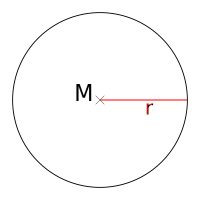
\includegraphics[width=.4\textwidth]{img/euclidean_circle.png}}\qquad
  \subfloat[][Taxicab-Kreis]{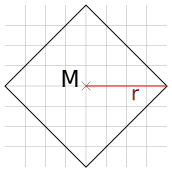
\includegraphics[width=.4\textwidth]{img/taxicab_circle.png}}\\
  \caption{Alle Punkte auf der Kreislinie haben den gleichen Abstand zum Mittelpunkt.
  Auffallend ist, das der Kreis in Taxicab-Metrik nicht rund, sondern quadratisch ist.}
  \label{img:circle_in_diff_metrics}
\end{figure}

Die Berechnung von Mittelpunkt und Radius eines Taxicab-Kreises ist schwieriger als in euklidischer 
Geometrie. Es wird hier keine Formel benutzt, sondern ein Algorithmus. Interessant hier ist das Berechnen
von einem Kreis in Taxicab-Geometrie von zwei oder drei Punkten. Das Problem lässt sich auch wie folgt
beschreiben: Finde das kleinste Quadrat, welches um \unit[45]{\textdegree} gedreht ist, welches zwei (drei) Punkte 
enthält. Da es nicht eindeutig definiert wird, reicht eine einzige Lösung für dieses Problem.

\begin{algorithm}[H]
    \caption{Kreis von zwei Punkten in Taxicab-Geometrie}
    \KwData{Zwei Punkte $X, Y \in \mathbb{R}^n$ }
    \KwResult{Radius und Mittelpunkt eines Quadrates, das $X$ und $Y$ enthält und eine minimale Seitenlänge hat.
    Radius hier ist die halbe Länge der Diagonale.}
    \BlankLine
    \begin{enumerate}
    \item Um die Lösung des Problems zu vereinfachen, werden die Punkte je um \unit[45]{\textdegree} um den
    Ursprung herum gedreht, dann das Quadrat berechnet, die so enstandende Lösung schließlich zurückgedreht.
    \item Rotiere $X, Y$ \unit[45]{\textdegree} um den Ursprung und nenne die so entstehenden Punkte $P, Q$.
    \item Offensichtlich ist nun die Seitenlänge $s$ des minimalen Quadrates gegeben durch
    \begin{equation*}
    s = \max\{|P_x - Q_x|, |P_y - Q_y|\}
    \end{equation*}
    \item Um eine Lösung zu finden, wähle die unterste linke Ecke als Ausgangspunkt und nenne sie $A$.
    \begin{equation*}
    \begin{cases}
    A_x = \min\{P_x,Q_x\}\\
    A_y = \min\{P_y,Q_y\}
    \end{cases}
    \end{equation*}
    \item Der rotierte Mittelpunkt $M'$ ist somit gegeben durch
    \begin{equation*}
    \begin{cases}
    M'_x = A_x + \frac{s}{2}\\
    M'_y = A_y + \frac{s}{2}
    \end{cases}
    \end{equation*}
    \item Rotiere $M'$ um \unit[-45]{\textdegree} um den Ursprung und nenne den so entstehenden Punkt $M$.
    \item Der Radius $r$ ist gegeben durch 
    \begin{equation*}
    r = \sqrt{A_x - M'_x) ^ 2 + (A_y - M'_y) ^ 2 }
    \end{equation*}
    \end{enumerate}
    \Return{$r$, $M$}
\end{algorithm} 

\begin{figure}[htb]
  \centering
  \subfloat[][Zwei Punkte]{\includegraphics[width=.45\textwidth]{img/taxicab_from_two.png}}\qquad
  \subfloat[][Drei Punkte]{\includegraphics[width=.45\textwidth]{img/taxicab_from_three.png}}\qquad
  \caption{Kreis in Taxicab-Geometrie von zwei respektiv drei Punkten. Auffallend ist, dass mindestens
  zwei Punkte auf der Kreislinie liegen.}
  \label{fig:taxicab_calc}
\end{figure}

Interessanterweise liefert dieser Algorithmus durch geringfügige Anpassungen auch die Lösung für folgendes Problem:
Finde das kleinste Quadrat, welches um \unit[45]{\textdegree} gedreht ist, welches \textbf{drei} Punkte enthält:

\begin{algorithm}[H]
    \caption{Kreis von drei Punkten in Taxicab-Geometrie}
    \KwData{Drei Punkte $X, Y, Z \in \mathbb{R}^n$ }
    \KwResult{Radius und Mittelpunkt eines Quadrates, das $X, Y, Z$ enthält und eine minimale Seitenlänge hat. Radius hier 
    ist die halbe Länge der Diagonale.}
    \BlankLine
    \begin{enumerate}
    \item Um die Lösung des Problems zu vereinfachen, werden die Punkte je um \unit[45]{\textdegree} um den
    Ursprung herum gedreht, dann das Quadrat berechnet, die so enstandende Lösung schließlich zurückgedreht.
    \item Rotiere $X, Y, Z$ \unit[45]{\textdegree} um den Ursprung und nenne die so entstehenden Punkte $P, Q, R$.
    \item Offensichtlich ist nun die Seitenlänge $s$ des minimalen Quadrates gegeben durch
    \begin{equation*}
    s = \max\{|P_x-Q_x|,|P_x-R_x|,|Q_x-R_x|,|P_y-Q_y|,|P_y-R_y|,|Q_y-R_y|\}
    \end{equation*}
    \item Um eine Lösung zu finden, wähle die unterste linke Ecke als Ausgangspunkt und nenne sie $A$.
    \begin{equation*}
    \begin{cases}
    A_x = \min\{P_x,Q_x,R_x\}\\
    A_y = \min\{P_y,Q_y,R_y\}
    \end{cases}
    \end{equation*}
    \item Der rotierte Mittelpunkt $M'$ ist somit gegeben durch
    \begin{equation*}
    \begin{cases}
    M'_x = A_x + \frac{s}{2}\\
    M'_y = A_y + \frac{s}{2}
    \end{cases}
    \end{equation*}
    \item Rotiere $M'$ um \unit[-45]{\textdegree} um den Ursprung und nenne den so entstehenden Punkt $M$.
    \item Der Radius $r$ ist gegeben durch 
    \begin{equation*}
    r = \sqrt{A_x - M'_x) ^ 2 + (A_y - M'_y) ^ 2 }
    \end{equation*}
    \end{enumerate}
    \Return{$r$, $M$}
\end{algorithm}

Im Rahmen dieser Arbeit wurden diese Algorithmen auch mittels GeoGebra visualisiert. Eine interaktive Visualisierung
für einen Kreis in Taxicab-Geometrie, der zwei (drei) Punkte enthält, ist unter folgenden Links zu sehen: 

\url{http://www.geogebratube.org/student/m65241} \newline
\url{http://www.geogebratube.org/student/m68655}

Interessanterweise funktioniert \texttt{minidisk} auch mit Taxicab-Kreisen, wenn man die \texttt{disk}-Funktion anpasst. Dies wurde hier nicht mathematisch bewiesen, aber die Ergebnisse sprechen für sich.

\begin{figure}[!ht]
  \centering
  \includegraphics[width=.9\textwidth]{img/taxicab_minidisk.png}
  \caption{Platzierung von 100 Punkten und deren kleinster umschließender Kreis in Taxicab-Geometrie.}
  \label{img:taxicab_minidisk}
\end{figure}

%#
\subsection{Zeitbeschränkung}

Das Einhalten Zeitbeschränkung ist nun trivial. Da es einen festen Treffpunkt gibt, sind nur Bewegungen in Zellen erlaubt, die einen 
Abstand von gleich oder weniger als dem Wert der verbliebenen Schritten haben. Mit jedem neuen Schritt wird dieser Kreis
um den Treffpunkt kleiner, und die Roboter treffen sich zwangsläufig in einem Punkt. Ein Schritt hier ist vollzogen, wenn alle Roboter ihren Zug gemacht haben (Bewegung in benachbarte Zelle oder NOP).

% ############################################
\clearpage
\section{Implementierung}

Die Implementierung beruht auf der Modellierung der Umgebung als Gitter von quadratischen Zellen. Zunächst wird, wie zuvor beschrieben, Missionsdauer und Ziel bestimmt. Falls mit der doppelten Missionsdauer gerechnet werden soll, muss \texttt{steps} einfach verdoppelt werden. In jedem Schritt werden die Roboter nacheinander bewegt. Wichtig ist hier, das in-place gearbeitet wird, damit für jeden Roboter die Invariante aus (\ref{eq:robot_constraint}) gilt. Ein Roboter macht einen Schritt und guckt auf die Positionen der anderen Roboter und macht dann seinen Zug. Der nächste Roboter betrachtet dann die neue Position des zuvor berechneten Roboters. Da bei einem Zug beachtet wird, dass er legal sein muss (kann Ziel erreichen und Roboter in der Nähe), bleibt diese Invariante auch invariant.

Die eigentliche Logik ist in der \texttt{agent}-Funktion. Diese aktualisiert den Wert des gesammelten Mangans und der gelaufenen Strecke. Viel wichtiger ist aber, dass dort entschieden wird, ob und in welche Zelle sich ein Roboter bewegt.

\begin{algorithm}[H]
    \caption{Mangan Harvest}  
    \KwData{Menge von Robotern $R$}
    \KwResult{}
    \BlankLine
    circle \textleftarrow  minidisk(R)\;  
    steps \textleftarrow  radius(circle)\;
    goal \textleftarrow center(circle)\; 
 
    \For{$t \leftarrow 1$ \KwTo steps} {
      timeleft \textleftarrow steps - t;
      \For{$n \leftarrow 1$ \KwTo $|R|$} {
        agent(n, timeleft);
      }
    }
    \Return{$R$}

\end{algorithm} 

\subsection{Logik}

Jeder Roboter soll eigens mit seinen Sensoren seine Umgebung erfassen und daraus
eine rationale Entscheidung treffen. Dabei kann er andere Roboter sowie
geerntete und ungeerntere Felder in einem Umkreis von 200 Metern erfassen. Eine
Entscheidung beinhaltet den nächsten Zug in eine der benachbarten quadratischen
Zellen, sodass jeder Roboter bis zu 4 Auswahlmöglichkeiten pro Zug besitzt.

\subsubsection{Heuristic Agent}
Der verfolgte Lösungsansatz eines Heuristic Agent lässt sich in drei Heuristiken 
gliedern. Eine Heuristik hier ist etwas wie eine Daumenregel, eine Entscheidungshilfe,
von der man ausgeht, dass sie gute Ergebnisse liefert.

\begin{enumerate}
\item Von einen Set aller benachbarten Zellen, die besucht werden können, filtere
jene Zellen heraus, die noch nicht geerntet wurden. Falls alle Zellen bereits
geerntet sind, behalte alle Zellen im Set.
\item Falls mehr als eine Zelle zur Auswahl steht, wähle jene Zellen, bei der die
Richtung in die sich bewegt wird eine höhere Dichte and ungeernteten Zellen
aufweist. Dazu wird ein quadratisches Feld von definierbarer größe wie in
Abbildung [ref] vor dem Roboter auf gebaut und berechnet wie viele ungeerntete
Zellen in diesem Feld vorhanden sind. Ebenfalls wirkt sich ein anderer Roboter,
der sich in diesem Feld befindet negativ auf die Gewichtung aus. Schließlich
werden ein oder mehrere Felder mit der höchsten Dichte an ungeernteten Feldern
ausgewählt und die dazugehörigen Zellen in die Entscheidungsfindung weiter
aufgenommen.
\item Falls mehr als eine Zelle zur Auswahl steht, wähle jene Zelle, die die
Distanz zu den umstehenden Robotern maximiert. Dazu werden die Zellen gefiltert,
welche die Distanz zum naheligensten Roboter maximieren. Falls es mehr als eine
Zelle ist, wird die Distanz zum zweitnähesten Roboter maximiert usw.
\item Falls mehr als eine Zelle zur Auswahl steht (zu diesem Zeitpunkt eher
unwahrscheinlich), eine beliebige Zellen aus den Entscheidungsmöglichkeiten.
\end{enumerate}

\begin{figure}
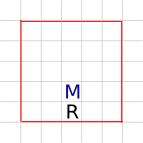
\includegraphics[width=.4\textwidth]{img/heuristic_density.png}
\centering
\caption{Schritt 2 des Heuristic Agent \\R - Roboter M - Zug, der auf Dichte untersucht wird \\ Roter Bereich - Quadrat der Größe 5, dessen Zellen in die Dichteberechnung einfließen}
\end{figure}

\subsection{Collected}

Da auf Genauigkeit Wert gelegt wird, wird nicht nur berechnet, wie viele Zellen ein Roboter besucht hat, um auf die gesammelten Manganmenge zu schließen. Wenn ein Roboter eine Zelle verlässt und in eine Benachbarte wechselt, so überstreicht sein Arbeitsbereich auch die Ecken. Dieser Vorgang ist in Fig. \ref{fig:harvested_edges} dargestellt. 

Die gesammelte Menge an Mangan $M [kg]$  berechnet sich wie folgt:

\begin{equation*}
M = |Z| \times \frac{\pi}{4} + |E| \times \frac{4-\pi}{16}
\end{equation*}

wobei $Z$ die Menge an besuchten Zellen ist, und $E$ die Menge an überstrichenen Ecken (keine Duplikate). Hintergrund ist hier, 
dass der Innenkreis einen Anteil von $\frac{\pi}{4}$ an der Zelle hat, somit jede Ecke $ \frac{1}{4} \times (1- \frac{\pi}{4}) $.

\begin{figure}[!ht]
  \centering
  \subfloat[][]{\includegraphics[width=.4\textwidth, angle=0]{img/collected_edges.png}} \qquad
  \subfloat[][]{\includegraphics[width=.4\textwidth, angle=90]{img/collected_edges.png}}\\
  \subfloat[][]{\includegraphics[width=.4\textwidth, angle=180]{img/collected_edges.png}} \qquad
  \subfloat[][]{\includegraphics[width=.4\textwidth, angle=270]{img/collected_edges.png}}
  \caption{Überstreichen der Ecken beim Wechseln in eine benachbarte Zelle: Der Roboter (hier rot),
  kann nicht nur den ursprünglichen, kreisförmigen Teil in der Mitte einer Zelle abernten, 
  sondern beim Wechseln auch die Ecken, da sein Arbeitsbereich diese in der Bewegung überschneidet. }
  \label{fig:harvested_edges}
\end{figure}


% ############################################
\clearpage
\section{Diskussion}

\subsection{Performance}

Die Zeit für Berechnungen ist kaum zu merken; am Längsten dauert noch die Visualisierung. Die einzige Einschränkung, die es der Zahl zu simulierenden Robotern gibt, ist die Zeit, die man warten möchte. 

\subsection{Fehlerrechnung}

\subsubsection{Fehler durch Modellierung}

In der Modellierung selbst gibt es keine Fehler, wie es zum Beispiel durch Annäherung der kreisförmigen Arbeitsbereiche durch Polygone der Fall wäre.

\subsubsection{Abweichung von der Optimalen Lösung}

Die maximale Menge an Mangan $M_max$, die gesammelt werden kann, lässt sich wie folgt berechnen:

\begin{equation*}
M_max = |R| \times T
\end{equation*}

wobei T die Missionsdauer ist. Im Folgenden wird für verschiedene Szenarien jeweils die prozentuale Zielereichung aufgezeigt. Diese Dateien entsprechen denen, die abgegeben wurden.

\begin{figure}[h!]
\centering
\begin{tabular}{ l|l|l }
n   & Single &  Double   \\ \hline
4   & 99.61 & 99.68 \\
10  & 94.84 & 97.24 \\
50  & 78.91 & 91.08 \\
100 & 88.74 & 91.77 \\
\end{tabular}
\caption{Erreichung des Optimums in \% \\ für verschiedene Anzahl von Robotern }
\end{figure}

\newpage

\nocite{*}

\printbibliography[maxnames=25]



\end{document}
